\section{Extension to Other Error Models}
In many cases {FLE} cannot be properly modelled as an isotropic, independent, random variable. In the case of optical tracking systems for example \cite{736031} the errors normal to the camera plane are approximately 3 times those parallel to the camera plane. It is straightforward to implement such an anisotropic \gls{FLE} in SciKit-SurgeryFRED and test the effect on registration outcomes.

Listing 1 shows a snippet taken from the function main.getfle(). The second line defines the ratio of \gls{FLE} in three directions. By default they are all one, but in the example shown in Listing 1 the error in the x direction has been set to be three times that in the y and z directions. 

\begin{pythonlisting}{\label{lis:anis} Code snippet for anisotropic {FLE}}
    fle_sd = np.random.uniform(low=0.5, high=5.0)
    fle_ratio = np.array([3.0, 1.0, 1.0], dtype=np.float64)
    anis_scale = math.sqrt(3.0 / (np.linalg.norm(fle_ratio) ** 2))
    fixed_fle = fle_ratio * fle_sd * anis_scale
\end{pythonlisting}
\begin{figure}
	\begin{center}
	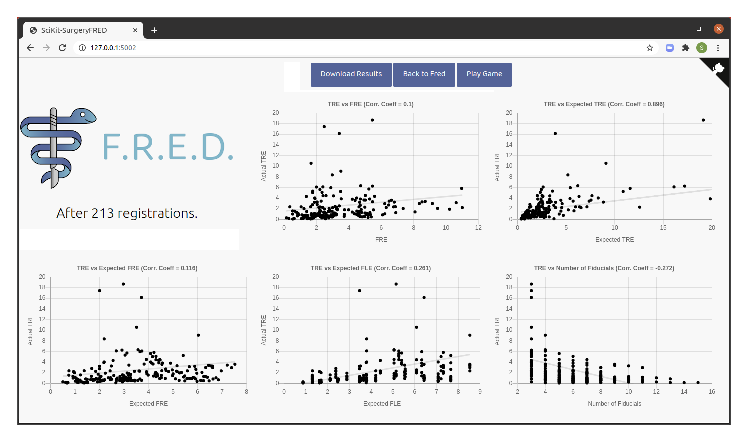
\includegraphics[width=0.7\linewidth]{images/anisitropic_error.eps}
		\caption{\label{fig:anis_errors}Results of 203 registrations using an anisotropic model of {FLE}. The error in the x direction was scaled to be three times that in the y and z directions.}
	\end{center}
\end{figure}

\begin{javalisting}{Java to generate independent FLE}
function clearCanvas(canvas) {
  if (canvas.getContext) {
    var ctx = canvas.getContext('2d');
    ctx.clearRect(0, 0, canvas.width, canvas.height);
  }
}
\end{javalisting}

